\documentclass[aspectratio=169]{beamer}
% \usepackage{enumitem}
\usepackage[utf8]{inputenc}
\usepackage{amsmath, amssymb, amsthm}
\usepackage{algorithm2e}
\usepackage{tikz}
\usepackage{amsmath, amsthm, amssymb}
\usepackage{pgfplots}
\newcommand{\hs}[1]{\hspace*{#1cm}}
\newcommand{\vs}[1]{\vspace*{#1cm}}

\title{Adversarial Uncertainty Quantification in Physics-Informed Neural Networks}
\author{Yibo Yang, Paris Perdikaris}
\institute{University of Pennsylvania}
\date{26.05.2023}

\begin{document}

\maketitle

\section{Introduction}

\begin{frame}{The model: UQPINN}
\begin{minipage}{0.6\textwidth}
{\huge UQPINN = GAN + PINN}
\end{minipage}\hfill
\begin{minipage}{0.4\textwidth}
\begin{enumerate}
    \item \textbf{UQPINN} : Uncertainty Quantification Physics-Informed Neural Network
    \item \textbf{GAN} : Generative Adversarial Network
    \item \textbf{PINN} : Physics-Informed Neural Network
\end{enumerate}
\end{minipage}
\end{frame}

\begin{frame}{Novalty}
"we will develop a flexible \textcolor{orange}{variational inference} framework 
that will allow us to train such models directly from \textcolor{orange}{noisy input/output data}, 
and predict outcomes of non-linear dynamical systems that are partially \textcolor{orange}{observed}
with quantified \textcolor{orange}{uncertainty}"
\hs{1}
\begin{flushright}
    \textit{-- Yibo Yang, Paris Perdikaris}
\end{flushright}
\hs{2}

\uncover<2->{
    \centering
    Using adversarial approach to handle randomness in observations.  
}

\end{frame}

\begin{frame}{GAN}

\begin{minipage}{0.5\textwidth}
    \begin{tikzpicture}[]
        \only<1,4-5>\draw[fill=brown] (0.5, 1) -- (2, 1.5) -- (2, 2.5) -- (0.5, 3) -- cycle;
        \only<1-3>\draw[fill=cyan] (3, 2.5) -- (4.5, 2) -- (4.5, 4) -- (3, 3.5) -- cycle;
        \only<1,4-5>\draw[->] (2, 2) .. controls (2.5, 2) and (3, 2) .. (3, 3);
        \only<1-3>\draw[->] (2, 4) .. controls (2.5, 4) and (3, 4) .. (3, 3);
        \only<1,4-5>\draw[->] (0, 2) -- (0.5, 2);
        \only<1-3>\draw[->] (4.5, 3) -- (5, 3);
        \only<1,4-5>\draw[] node at (-0.7, 2) {$z\sim p(z)$};
        \only<1,4-5>\draw[] node at (2.5, 1.5) {$p_\theta(x)$};
        \only<1-3>\draw[] node at (1.7, 4) {$q(x)$};
        \only<1-3>\draw[] node at (5.2, 3) {$\rho$};
        \only<1,4-5>\draw[] node at (1, 2) {$f_\theta$};
        \only<1-3>\draw[] node at (3.5, 3) {$T_\psi$};
        \only<1,4-5>\draw[] node at (1.2, 0.7) {generator};
        \only<1-3>\draw[] node at (3.9,1.8) {discriminator};
        % \draw[step=0.5, black, thin] (0,0) grid (5, 5); 
        % \foreach \i in {0,0.5,...,5.0} {
		%     \draw [very thin, gray] node [below] at (\i,0) {$\i$};
        %     \draw [very thin, gray] node [left] at (0,\i) {$\i$};
        % }
    \end{tikzpicture}
\end{minipage}\hfill
\begin{minipage}{0.5\textwidth}
\only<1>{
    \begin{align*}
        & \underset{\psi}{max}~\mathcal L_{\mathcal D}(\psi)
        \\
        & \underset{\theta, \phi}{min}~\mathcal L_{\mathcal G}(\theta, \phi) + \beta~\mathcal L_{PDE} (\theta)
    \end{align*}
}
\only<2-3>{
    \begin{align*}
        \underset{\psi}{argmin}&\frac{\rho(y=+1|x,t,u)}{\rho(y=-1|x,t,u)}
        \\
        p_\theta(x,t,u) &= \rho(x,t,u|y=+1)
        \\
        q(x,t,u) &= \rho(x,t,u|y=-1)
    \end{align*}
}
\only<3>{

    $$T_\psi \approx \rho(y=+1|x,t,u)$$
  
    \begin{align*}
        \mathcal L_D(\psi) &= \mathbb E_{q(x,t)p(z)}[log ~\sigma(T_\psi(x,t,f_\theta))] 
        \\
        &+\mathbb E_{q(x,t,u)}[log(1-\sigma(T_\psi))]
    \end{align*}
}
\only<4-5>{
    \begin{align*}
        \underset{\theta}{argmax}~\mathbb{KL}\left[
        p_\theta(x,t,u)
        \Vert
        q(x,t,u)\right]
    \end{align*}
}
\only<5>{
    \begin{align*}
        \mathcal L_G(\theta,\psi) &= \mathbb E_{q(x,t)p(z)}
[T_\psi(x,t,f_\theta(x,t,z))
\\
&+(1-\lambda )log(q_\phi(z|x,t,f_\theta(x,t,z)))]
    \end{align*}
}
\end{minipage}

\end{frame}

\section{Experiment}

\begin{frame}{Experiment Setup}
\begin{tabular}{p{0.2\textwidth}p{0.4\textwidth}p{0.4\textwidth}}
    &{\Large Author's Experiment Setup} & \uncover<2->{\Large My Experiment Setup}\\[0.5cm]

    \textbf{GPU} & NVIDIA Tesla P100(16GB) & \uncover<2->{MX450(2GB)}\\[0.2cm]
    
    \textbf{DL framework} & Tensorflow v1.10 & \uncover<2->{Pytorch v1.9.0}\\[0.2cm]
   
    \textbf{Formula} & \begin{enumerate}
        \item pedagogical ODE
        \item Burgers' equation
        \item Darcy flow
    \end{enumerate} & \uncover<2->{\begin{enumerate}
        \item pedagogical ODE
        \item Burgers' equation
        \item Darcy flow
    \end{enumerate}}\\
    
    \textbf{Model} & UQPINN & \uncover<2->{\begin{enumerate}
        \item UQPINN
        \item PINN
    \end{enumerate}}\\
\end{tabular}

\uncover<3->{    
\centering
    parameters are set to be the same as the author's
}
\end{frame}

\begin{frame}{pedagogical ODE}
%  % This file was created with tikzplotlib v0.10.1.
\begin{tikzpicture}

\definecolor{darkslategray38}{RGB}{38,38,38}
\definecolor{lavender234234242}{RGB}{234,234,242}
\definecolor{lightgray204}{RGB}{204,204,204}
\definecolor{peru22113282}{RGB}{221,132,82}
\definecolor{steelblue76114176}{RGB}{76,114,176}

\begin{axis}[
axis background/.style={fill=lavender234234242},
axis line style={white},
legend cell align={left},
legend style={
  fill opacity=0.8,
  draw opacity=1,
  text opacity=1,
  draw=lightgray204,
  fill=lavender234234242
},
tick align=outside,
title={Losses},
x grid style={white},
xlabel=\textcolor{darkslategray38}{Iteration},
xmajorgrids,
xmajorticks=false,
xmin=-9.95, xmax=208.95,
xtick style={color=darkslategray38},
y grid style={white},
ylabel=\textcolor{darkslategray38}{Loss},
ymajorgrids,
ymajorticks=false,
ymin=-0.391387329250574, ymax=9.23482891991734,
ytick style={color=darkslategray38}
]
\addplot [semithick, steelblue76114176]
table {%
0 1.9748387336731
1 0.910723090171814
2 0.0461679548025131
3 0.558556318283081
4 0.714794278144836
5 0.491124838590622
6 0.812751531600952
7 1.58011162281036
8 0.664521157741547
9 1.74222671985626
10 2.30384302139282
11 2.54707789421082
12 2.92063498497009
13 3.21416902542114
14 3.22849369049072
15 3.63434219360352
16 3.60304880142212
17 2.57984209060669
18 2.01718664169312
19 1.78607201576233
20 1.62153244018555
21 1.47789132595062
22 1.37412559986115
23 1.28963971138
24 1.29018020629883
25 1.18847858905792
26 1.231853723526
27 1.12836849689484
28 1.06192946434021
29 1.03598260879517
30 1.02946615219116
31 0.927079796791077
32 0.917259693145752
33 0.865631818771362
34 0.877282917499542
35 0.848894000053406
36 0.836766481399536
37 0.820337176322937
38 0.855978012084961
39 0.863053560256958
40 0.802315354347229
41 0.858992218971252
42 0.823311746120453
43 0.916647672653198
44 0.949414849281311
45 0.911380171775818
46 0.940291106700897
47 0.930164098739624
48 0.928079962730408
49 0.980206072330475
50 0.367721378803253
51 0.87900972366333
52 0.639588475227356
53 0.703643918037415
54 0.833283841609955
55 0.75062507390976
56 0.89892303943634
57 0.869606375694275
58 0.942725360393524
59 0.882761061191559
60 0.898633360862732
61 0.932310223579407
62 0.961142599582672
63 0.978223562240601
64 1.09392547607422
65 1.11103427410126
66 1.1744225025177
67 1.23731899261475
68 1.41566181182861
69 1.52388286590576
70 1.56807434558868
71 1.60424447059631
72 1.65365135669708
73 1.67136573791504
74 1.89047968387604
75 1.92959880828857
76 1.99458205699921
77 2.02426743507385
78 2.06378436088562
79 2.17548561096191
80 2.2188994884491
81 2.28466176986694
82 2.32412338256836
83 2.30534529685974
84 2.34409284591675
85 2.51692581176758
86 2.60399913787842
87 2.69612812995911
88 2.69597434997559
89 2.78733158111572
90 2.84786105155945
91 2.86836743354797
92 2.86462783813477
93 3.00384664535522
94 3.07514810562134
95 3.06723189353943
96 3.16557216644287
97 3.24764204025269
98 3.27929377555847
99 3.26273655891418
100 3.30093002319336
101 3.42290925979614
102 3.50645017623901
103 3.5116024017334
104 3.56242394447327
105 3.61044859886169
106 3.64226007461548
107 3.67048740386963
108 3.7054328918457
109 3.71596169471741
110 3.85562801361084
111 3.83216142654419
112 3.93104839324951
113 3.83490896224976
114 3.91870188713074
115 3.95068025588989
116 3.94071340560913
117 3.97391080856323
118 3.99679398536682
119 4.08423376083374
120 4.07750701904297
121 4.14800357818604
122 4.14057207107544
123 4.08700037002563
124 4.14499473571777
125 4.15958786010742
126 4.19741153717041
127 4.23107385635376
128 4.37979698181152
129 4.30614423751831
130 4.36740207672119
131 4.39232301712036
132 4.31655073165894
133 4.44118213653564
134 4.41542911529541
135 4.50745487213135
136 4.47615146636963
137 4.47195100784302
138 4.52286195755005
139 4.57901096343994
140 4.42842960357666
141 4.3132495880127
142 4.27264881134033
143 4.16028690338135
144 4.17050790786743
145 4.13832426071167
146 4.07220077514648
147 3.91368293762207
148 3.84680199623108
149 3.73428869247437
150 3.65027236938477
151 3.54485535621643
152 3.54496574401855
153 3.49003219604492
154 3.43221139907837
155 3.43308472633362
156 3.36478066444397
157 3.3830361366272
158 3.38997793197632
159 3.38422966003418
160 3.33655309677124
161 3.33020210266113
162 3.38178586959839
163 3.4674711227417
164 6.01458835601807
165 3.5087947845459
166 3.45937490463257
167 3.37549591064453
168 3.3909740447998
169 3.37572193145752
170 3.79881906509399
171 3.81236100196838
172 3.47810506820679
173 3.4316143989563
174 3.47533965110779
175 3.37924337387085
176 3.56363677978516
177 3.40421581268311
178 4.74012041091919
179 3.44659543037415
180 3.47532773017883
181 3.40569686889648
182 8.79727363586426
183 7.40422773361206
184 7.37381076812744
185 7.26069116592407
186 7.03100872039795
187 6.91180992126465
188 5.97824287414551
189 5.94848680496216
190 5.94538021087646
191 5.92880439758301
192 5.96929597854614
193 6.06565618515015
194 5.98967504501343
195 5.92999029159546
196 5.90889739990234
197 5.85291433334351
198 5.93437147140503
199 6.00430154800415
};
\addlegendentry{loss_G}
\addplot [semithick, peru22113282]
table {%
0 0.831904828548431
1 1.04735815525055
2 1.93143391609192
3 1.13470149040222
4 0.842112004756927
5 1.03640973567963
6 0.815528333187103
7 0.469484001398087
8 1.01276338100433
9 0.464154452085495
10 0.353756308555603
11 0.33501660823822
12 0.317400395870209
13 0.325187742710114
14 0.43817201256752
15 0.760511219501495
16 1.81280708312988
17 1.39067268371582
18 1.3131719827652
19 1.30214726924896
20 1.26809012889862
21 1.27460527420044
22 1.25752937793732
23 1.24544835090637
24 1.24523901939392
25 1.2394483089447
26 1.23815286159515
27 1.24317169189453
28 1.24546074867249
29 1.24309062957764
30 1.23841655254364
31 1.23734712600708
32 1.23916614055634
33 1.24320495128632
34 1.24960458278656
35 1.24212169647217
36 1.24397587776184
37 1.23610484600067
38 1.23269414901733
39 1.22623193264008
40 1.21620976924896
41 1.20683085918427
42 1.19867753982544
43 1.18166530132294
44 1.17438328266144
45 1.16032648086548
46 1.1505833864212
47 1.13325417041779
48 1.1596052646637
49 1.14375960826874
50 1.4696558713913
51 1.26595640182495
52 1.29685080051422
53 1.06452250480652
54 1.33315849304199
55 1.14029955863953
56 1.26866292953491
57 1.1038213968277
58 1.15196573734283
59 1.07324492931366
60 1.09366512298584
61 1.11804032325745
62 1.00197553634644
63 1.04972851276398
64 1.05452156066895
65 1.02701103687286
66 0.925058662891388
67 0.924061834812164
68 0.899560570716858
69 0.962006747722626
70 0.97472757101059
71 0.871675610542297
72 0.844704151153564
73 0.863736689090729
74 0.829027354717255
75 0.896343946456909
76 0.82721745967865
77 0.821205615997314
78 0.791440367698669
79 0.868966460227966
80 0.7945436835289
81 0.768618106842041
82 0.771819651126862
83 0.76032692193985
84 0.748661041259766
85 0.738629341125488
86 0.702594041824341
87 0.738013625144958
88 0.761845767498016
89 0.712130188941956
90 0.713120877742767
91 0.725794970989227
92 0.723945558071136
93 0.676356256008148
94 0.721637368202209
95 0.698358118534088
96 0.676644206047058
97 0.683376550674438
98 0.689153790473938
99 0.703122794628143
100 0.670400321483612
101 0.638146042823792
102 0.67233669757843
103 0.69842129945755
104 0.680824041366577
105 0.666061043739319
106 0.660162150859833
107 0.659687995910645
108 0.654113948345184
109 0.652387022972107
110 0.658775925636292
111 0.652814745903015
112 0.647771775722504
113 0.660211086273193
114 0.657424628734589
115 0.637131989002228
116 0.668312907218933
117 0.677700400352478
118 0.662386357784271
119 0.677398860454559
120 0.679326832294464
121 0.677788376808167
122 0.649829387664795
123 0.642110645771027
124 0.678626477718353
125 0.688843905925751
126 0.656753182411194
127 0.666940093040466
128 0.656803667545319
129 0.661558032035828
130 0.649387955665588
131 0.659984767436981
132 0.686679065227509
133 0.674648821353912
134 0.69710111618042
135 0.691699922084808
136 0.702632427215576
137 0.716756999492645
138 0.729133009910583
139 0.761009156703949
140 0.805651068687439
141 0.830973088741302
142 0.827361583709717
143 0.86371511220932
144 0.887420833110809
145 0.894026756286621
146 0.913860023021698
147 0.927156865596771
148 0.943602085113525
149 0.956211268901825
150 0.962305128574371
151 0.97547173500061
152 0.976769804954529
153 0.960254728794098
154 0.957559764385223
155 0.948835670948029
156 0.949777245521545
157 0.942382633686066
158 0.940717577934265
159 0.949896931648254
160 0.954194247722626
161 0.953580379486084
162 0.944075345993042
163 0.951594412326813
164 0.650250792503357
165 0.955837309360504
166 0.948097825050354
167 0.949208319187164
168 0.943114042282104
169 0.942530572414398
170 0.937302887439728
171 0.944639325141907
172 0.944031536579132
173 0.947326123714447
174 0.953545212745667
175 0.937714755535126
176 0.936927318572998
177 0.935622155666351
178 0.782062768936157
179 0.944882452487946
180 0.926490783691406
181 0.943574786186218
182 0.525165975093842
183 0.440435320138931
184 0.420304208993912
185 0.412186980247498
186 0.386950463056564
187 0.368139922618866
188 0.378781318664551
189 0.38587087392807
190 0.368483185768127
191 0.355620533227921
192 0.373500615358353
193 0.352524846792221
194 0.369651436805725
195 0.375380456447601
196 0.353998184204102
197 0.367245346307755
198 0.375683069229126
199 0.364816308021545
};
\addlegendentry{loss_D}
\end{axis}

\end{tikzpicture}

$$
\begin{aligned}
\frac{\partial^2 u}{\partial x^2} &- u^2 \frac{\partial u}{\partial x}  f(x) & x&\in[-1,1]
\\
f(x) &= -\pi^2 sin(\pi x) - \pi cos(\pi x)sin(\pi x)^2
\\
u(x) & \sim \mathcal N(sin(\pi), noise)& x&=\{-1,1\}
\end{aligned}
$$
\end{frame}

\end{document}